%\documentclass[useAMS, usenatbib,usegraphicx,letter]{mn2e}
%\documentclass[11pt]{article}
\documentclass[reprint,aps,prd,superscriptaddress,showkeys,showpacs]{revtex4-1}
\usepackage{epsfig,amsmath,natbib}

\usepackage{aas_macros}
\usepackage{amssymb}
\usepackage{amsmath}
\usepackage{dsfont}
\usepackage{hyperref}
\usepackage{color}
\usepackage{pbox}
\usepackage{booktabs}

\hypersetup{
	colorlinks=false,
	citecolor=green
}
% \usepackage{graphicx}
% \usepackage{epstopdf}
% \usepackage{natbib}

%%%%%%%%%%%%%%%%%
%Custom commands%
%%%%%%%%%%%%%%%%%

\newcommand{\bb}[1]{\mathbf{#1}}
\newcommand{\bbh}[1]{\mathbf{\hat{#1}}}
\newcommand{\h}[1]{\hat{#1}}

%%%%%%%%%%%%%%%%%%%%%%%%%%%%%%%%%%%%%%%%%%%%%%

\begin{document}

\title{Weak Lensing simulations: the LensTools computing package}

\author{Andrea Petri}
\email{apetri@phys.columbia.edu}
\affiliation{Department of Physics, Columbia University, New York, NY 10027, USA}
\affiliation{Physics Department, Brookhaven National Laboratory, Upton, NY 11973, USA}

\date{\today}

\label{firstpage}

\begin{abstract}
Cosmosis at \citep{cosmosis}. The \texttt{SimulationBatch} class
    
\end{abstract}


\keywords{Weak Gravitational Lensing --- Simulations}
\pacs{98.80.-k, 95.36.+x, 95.30.Sf, 98.62.Sb}

\maketitle


%%%%%%%%%%%%%%%%%%%%%%%%%% INTRO %%%%%%%%%%%%%%%%%%%%%%%%%%%%%%%%%%%%%%%%%%%%%%%%%%%%%%%%

\section{Introduction}
%
Weak Gravitational lensing is a promising cosmological probe...  

%%%%%%%%%%%%%%%%%%% CODE %%%%%%%%%%%%%%%%%%%%%%%%%%%%%%%%%%%%%%%

\section{Code} 

\subsection{Shear field simulations}

\begin{figure*}
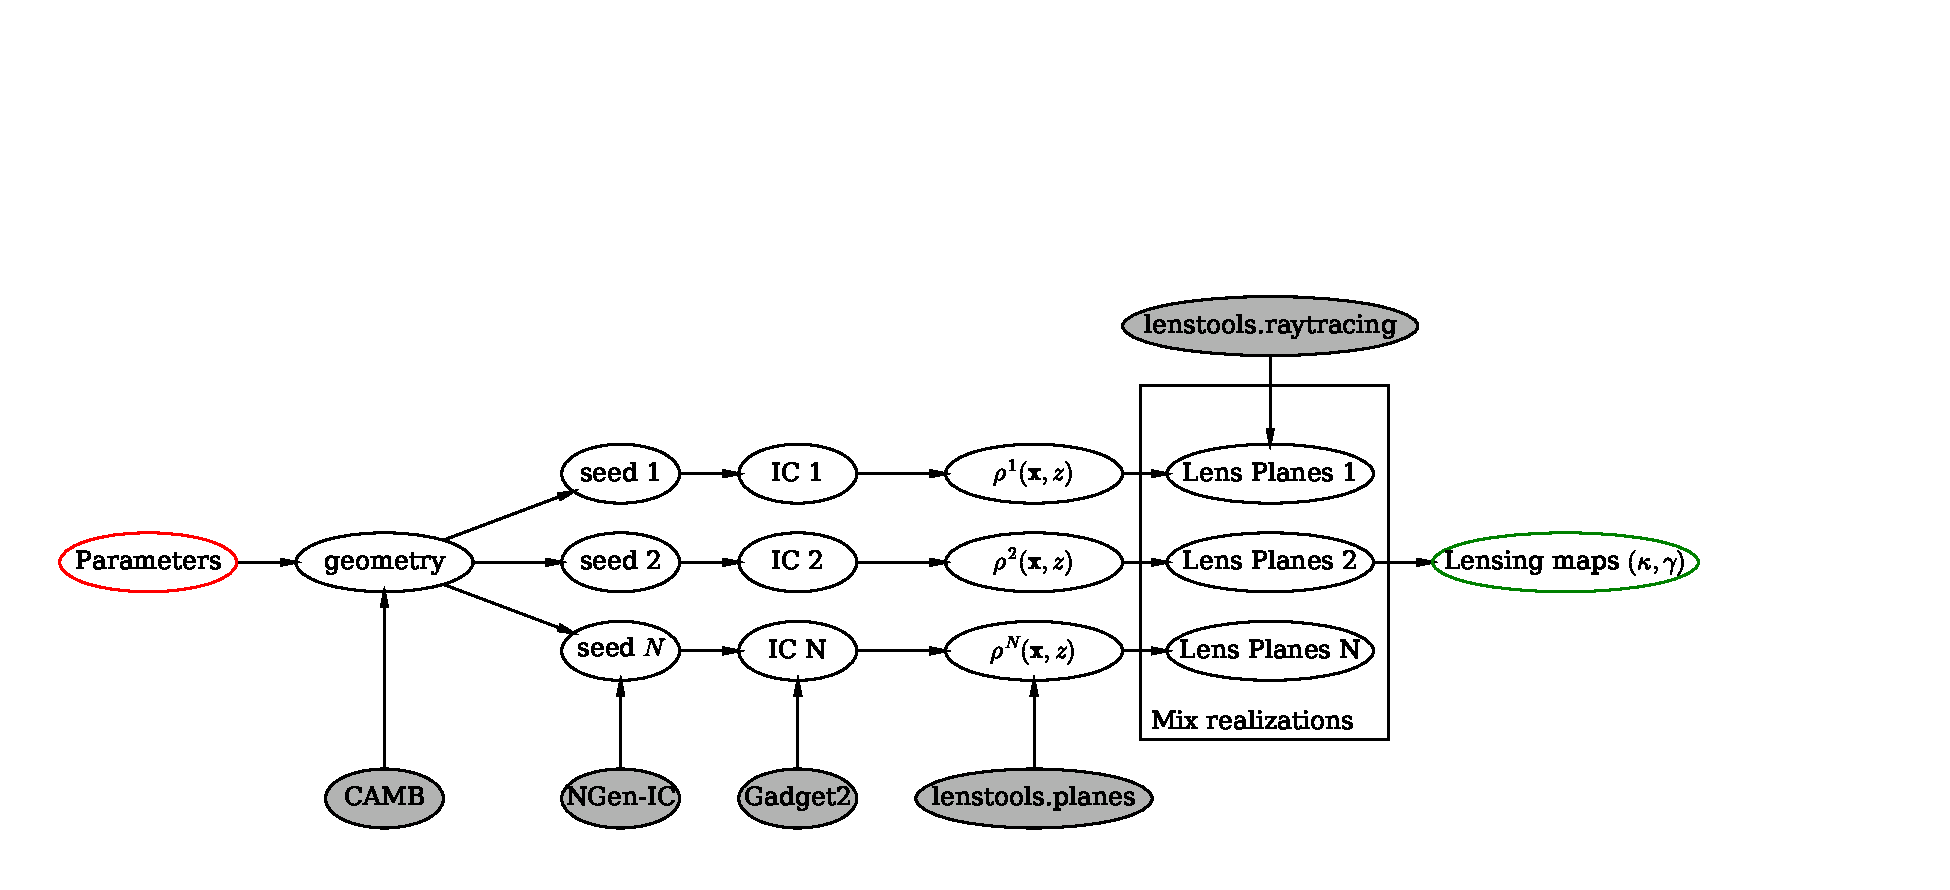
\includegraphics[scale=0.6]{Figures/flow.eps}
\end{figure*}

\subsection{Weak lensing features}

\subsection{Parameter estimation}

%%%%%%%%%%%%%%%%%%% EXAMPLES %%%%%%%%%%%%%%%%%%%%%%%%%%%%%%%%%%%%%%%

\section{Examples}

%%%%%%%%%%%%%%%%%% FUTURE %%%%%%%%%%%%%%%%%%%%%%%%%%%%%%%%%%%%%

\section{Future developments}

%%%%%%%%%%%%%%%%%% CONCLUSION %%%%%%%%%%%%%%%%%%%%%%%%%%%%%%%%%%%%%

\section{Conclusion}

%%%%%%%%%%%%%%%%%%%%%%%%%% ACKNOWLEDGMENTS %%%%%%%%%%%%%%%%%%%%%%%%%%%%%%%%%%%%%%%%%%%%%%%%%%%%%%
 

\section*{Acknowledgements}


\bibliography{ref}
\label{lastpage}
\end{document}
